\begin{center}
  \Large
  \textbf{BIOGRAFI PENULIS}
\end{center}

\addcontentsline{toc}{chapter}{BIOGRAFI PENULIS}

\vspace{2ex}

\begin{wrapfigure}{L}{0.3\textwidth}
  \centering
  \vspace{-3ex}
  % Ubah file gambar berikut dengan file foto dari mahasiswa
  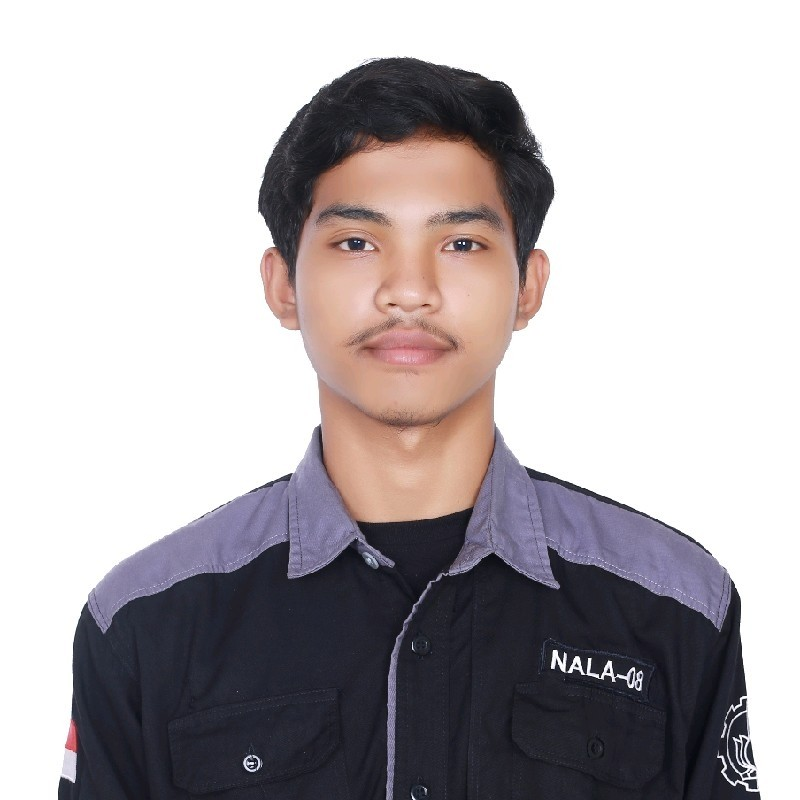
\includegraphics[width=0.3\textwidth]{gambar/my.jpg}
  \vspace{-4ex}
\end{wrapfigure}


Penulis menempuh pendidikan menengah di SMA Negeri Bali Mandara dan lulus pada tahun 2020. Pada tahun yang sama, penulis diterima sebagai mahasiswa Program Studi Teknik Komputer, Fakultas Teknologi Elektro dan Informatika Cerdas, Institut Teknologi Sepuluh Nopember (ITS) Surabaya. Selama masa studi di ITS, penulis aktif dalam berbagai kegiatan riset dan pengembangan teknologi. Penulis merupakan anggota tim robotika \emph{Barunastra ITS} yang berfokus pada pengembangan kapal otonom, dan berhasil meraih prestasi sebagai \emph{Juara 1 International Roboboat Competition 2023} di Florida, Amerika Serikat, serta \emph{Juara 1 Kontes Kapal Cepat Tak Berawak Nasional (KKCTBN)} dalam kategori \emph{Autonomous Tourism Surface Vehicle}.

Selain itu, penulis juga terlibat dalam proyek riset kendaraan otonom melalui pengembangan mobil tanpa pengemudi dalam tim \emph{ICar ITS}. Saat ini, penulis mengikuti program \emph{Apple Developer Academy} di Universitas Ciputra Surabaya guna memperdalam kompetensi di bidang pengembangan aplikasi digital. Penulis juga pernah menjalani program magang di \emph{PT Satkomindo Mediyasa} sebagai \emph{Full Stack Web Developer}, dengan tanggung jawab dalam pengembangan sistem ppendaftaran karyawan berbasis web. Penelitian tugas akhir ini diambil oleh penulis karena memiliki ketertarikan di bidang \emph{robotika}, pengembangan \emph{web}, dan \emph{machine learning}. Tugas akhir ini merupakan bagian dari riset pengembangan sistem \emph{robot quadruped-legged} untuk keperluan \emph{monitoring} infrastruktur kelistrikan di gardu induk menggunakan \emph{kamera termal}. Penelitian ini bagian dari kerja sama antara ITS, \emph{Ezra Robotics}, dan PLN dalam pengembangan teknologi robotika untuk pemantauan infrastruktur kelistrikan di Indonesia. Penulis berharap hasil penelitian ini dapat memberikan kontribusi positif bagi pengembangan teknologi robotika dan sistem pemantauan infrastruktur kelistrikan di Indonesia, serta menjadi referensi bagi penelitian selanjutnya dalam bidang yang sama. Selain itu Tugas Akhir ini disusun sebagai salah satu syarat untuk memperoleh gelar Sarjana Teknik (S.T.) di Program Studi Teknik Komputer, ITS Surabaya.